% !TEX root = MasterThesis.tex

\chapter{Case Study: Driver Development in Linux and Zircon}\label{ch:case-study}
Device drivers are an integral part of operating systems and require an in-depth understanding of the peripheral device and its controller, the hardware interface between device and computer abstraced by the target operating system from the developer.
The fundamental operating system principles and their realization were already established in the previous chapter.
But the question of what a device driver actually is and its responsibility was not discussed so far.
Therefore, answering these questions is a valid entry point to the actual case study about the driver models in Linux and Zircon and the exemplary device driver development.

A device driver's main purpose is providing an abstraction between user applications and peripheral devices\cite{glatz2015betriebssysteme}.
A typical developer should not have to think about the way a specific device is controlled.
Especially, as even devices from the same type differ in the exact way they are managed, it would require too much in-depth knowledge from application developers and make the resulting applications very error-prone.
Thus, it is the task of a driver as a part of an operating system to 
\begin{itemize}
    \item define an abstraction of a device to the system,
    \item build and maintain the connection between applications and certain peripherals, 
    \item initialize the peripheral controller and the device if it is needed,
    \item query the device state from the controller,
    \item log events,
    \item provide a consistent \ac{api} for all devices from the same type to the user,
    \item receive abstract application requests and translate them to commands which can be submitted to the device and
    \item transfer data from and to the device\cite{glatz2015betriebssysteme},~\cite{tanenbaum-modern-operating-systems}.
\end{itemize}
%
Driver development is very operating system dependent and has wide-ranging consequences.
While the decision if drivers are located in user or kernel space some further questions remain with the choice of an architecture, some further questions remain.
Some of them are about the way and point in time a driver is attached to the operating system.
For example if the driver must be known at compile time or if it is possible to attach it later during runtime\cite{tanenbaum-modern-operating-systems}.
In any case, each system should provide a unified but extensible device driver interface which supports various device types, even for those that were non-existing at the time the operating system was designed\cite{glatz2015betriebssysteme}.
The design of the interface could be specific to each device type or standardized for all drivers\cite{tanenbaum-modern-operating-systems}.
Furthermore, in almost every operating system specific driver model, it has to be ensured a driver is \textit{re-entrant}, which means a running driver must be safe if it is called from several processes at the same time, and also still safe if peripheral devices become added or removed while the computer is still running\cite{tanenbaum-modern-operating-systems}.
In order to avoid re-developing or duplicating driver parts that remain the same for devices of the same type, device drivers are often modeled and implemented as a hierarchical or layered model.
A widespread pattern is to split the implementation into a logical and a physical layer.
The logical one contains driver functionality which remains consistent between devices of the same type while the physical layer only takes care of device specific functionality\cite{tanenbaum-modern-operating-systems} 

% \section{Driver Models}
  
\section{Linux Driver Model}
\subsubsection*{Driver Types}
As already mentioned, drivers most importantly implement an abstraction of the communication with \ac{io} peripherals.
To do so, Linux provides more ways than commonly known.
The first one is via \textit{direct hardware access} as \textit{user-space driver}.
As known from the previous sections most \ac{io} related drivers and its operations are privileged.
But Linux offers a way for normal user applications (userspace) to access hardware without a classical driver.
This way of accessing the hardware is mostly used for video drivers which are incorporated into the \textit{X.Org display server}.
In order to obtain the necessary rights two systemcalls are needed: \texttt{iopl()} to change the privileged level and \texttt{ioperm()} to set the \ac{io} port permissions.
These calls can only be performed by a privileged Linux user or the \textit{root} user.
Compared to other options to access peripheral hardware, this one has the disadvantage that interrupts are not available at all and the user software may run into issues with demand paging.
So this option is possibly slower than a device driver in kernelspace, but for some tasks, like the already named \textit{X.Org server} is this kind of a accessing hardware more appropriate than a kernel driver\cite{lfd430},~\cite{glatz2015betriebssysteme}.

Another widely unknown and \ac{cpu} specific way to perform \ac{io} operations is using \textit{minimal operating system support} to access serial interfaces on x86-based \acp{cpu}.
In doing so, the kernel does not know anything about the exact device but about its \ac{io} interface\cite{glatz2015betriebssysteme}.
Thus, this variant is not handled further.
Instead, this work will focus on \ac{io} drivers in \textit{kernel-space}, the most common way device drivers in Linux are written.
This kind of driver is a part of the kernel's address space, running in the \ac{cpu}'s kernel mode and thus privileged.
User applications can access kernel drivers and thus the devices via common file operations like \texttt{open()}, \texttt{close()}, \texttt{read()} or \texttt{write()} as they are shown virtually as \textit{special files} in the device filesystem \texttt{/dev/}.
Together with the optional entries in the \texttt{/sys/} filesystem and the older ones in \texttt{/proc/} devices in those filesystems are categorized in a structured way, according to their types\cite{glatz2015betriebssysteme}.
Linux differentiates drivers in the mentioned block devices, character devices and network devices, but internally drivers are structured in \textit{subsystems} of similar device functionality like usb, network, bluetooth, gpio and many others\cite{quade2016Linux}. 

As indicated above \textit{character} and \textit{block device drivers} in Linux have filesystem entries which are associated with them.
Such a file node is the basic way to communicate with the driver from userspace.
The fundamental \texttt{/dev/} directory but also the \texttt{/sys/} and \texttt{/proc/} are virtual.
They do not require more disk space than the needed inodes.
A device is identified by a \textit{device number} which is composed of a \textit{major number} to identify the device itself and the \textit{minor number} to count the existing device instances\cite{lfd430}.
Device numbers are in most cases assigned by the \textit{udev} mechanism today.
A closer look at it and its relation to the \texttt{/sys/} filesystem follows.

\textit{Character devices}, no matter in which subsystem, have in common that they are well represented as data streams.
They provide only sequential access to their data and can be accessed just like a regular file including the standard file operations\cite{lfd430}.
The same applies to \textit{block devices}.
In contrast to character devices block devices are read and written only in multiples of their block-size.
Linux enables devices of this type to behave similar to character devices and transfer any number of bytes per time, too\cite{lfd430}.
Random data access is also allowed and the access to their data is usually cached.
One characteristic of block devices is the fact a \textit{filesystem} can be mounted on the device.
Thus, file operations are of course available on them.
Examples are hard drives or USB memory sticks\cite{lfd430}.
The third device class, \textit{network devices}, are entirely different.
They transfer \textit{packets} of data.
Network devices are not mapped as files or provide file operations.
Instead, they are most often identified by name (\texttt{eth0}, \texttt{wlan0}) and accessed via the \textit{Berkeley socket} interface\cite{lfd430}.

\subsubsection*{Driver Build Types}
Device drivers in Linux can be a static part of the kernel or a dynamically loadable \textit{module}.
In older versions, only a static integration was possible. That means all the possibly needed drivers must be present at compile time.
Thus, the kernel size increases but some drivers will not be used at all and to add a new driver a recompilation and a reboot is needed.
Current Linux kernels additionally allow dynamically loadable modules with optional parameters.
Reloading a driver during runtime without a reboot does not only save space, it is also useful for development.
It is only needed to recompile and reload a single module instead of the entire kernel including a system reboot\cite{quade2016Linux}.
However, the module has to be built for exactly the same kernel version as running in order to be loaded.
A module which is dynamically loaded via \texttt{insmod} respectively \texttt{modprobe} is, like built-in drivers, a part of the kernel's address space and running in kernel mode.
But as this module does a dynamic binding to the kernel's symbol table, it is only allowed to use a, in comparison to built-in drivers, restricted \ac{api}\cite{glatz2015betriebssysteme}.
However, being a part of the kernel's address space assigns drivers a special responsibility.
As there is no isolation between parts of the kernel, an errornously implemented driver may crash the entire system as a result.
Whether a driver should be build as a built-in driver or as a module has little impact on its implementation.
It does require little or no changes to the source at all to switch between them as it is mostly a build configuration\cite{lfd430}.

Module drivers are indeed useful, but not realizable for every device type.
Some drivers, e.g.\ specific \ac{cpu} controllers, must be present at a very early system stage to enable Linux to read from hard drives.
Writing such a driver as a module which needs to read from a hard drive to be loaded dynamically into the system is therefore not realizable\cite{quade2016Linux}.

\subsubsection*{Driver Interfaces}
Device drivers in general need to call Linux system functions to include themself into the kernel, i.e.\ methods to initialize respectively deinitialize the driver and the associated device, operating system triggered functions, e.g.\ interrupt handler functions, as well as user application triggered routines to enable the communication between user and device\cite{quade2016Linux}.
The latter ones also include the driver-side implementations for the standard \ac{io} \ac{api}, the file operations.
It should be implemented in a device-specific way for the operations that are meaningful for the device.
If there is no such behavior, it is preferred to implement only the meaningful operations, leaving the default behavior for the others and switching to a better suited interface for the device.
Besides the standard \ac{io} \ac{api}, there are e.g.\ communication or multimedia specific \acp{api} which are better more appropriate for devices of these kinds.
Often, these interfaces are defined in Linux but built based on the \texttt{ioctl()} call which is technically a part of the file operations\cite{quade2016Linux}.
\ac{io} control is an universal interface to define its own, device specific commands.
An \texttt{ioctl()} command is usually made from a number and the type of optional arguments.
However, the preferred way is to utilize the macros Linux provides and use them to define a command consisting of the number, the argument types, the size of the transferred data and their transfer direction\cite{quade2016Linux}.
This is the best way to verify \texttt{ioctl()} calls to a certain extent.
The calls defined for the use in \texttt{ioctl()}'s must be known in both, kernel and userspace.
Thus, these interface descriptions and corresponding datastructure definitions must be accessible from both sides.
Typically, they are found in \texttt{linux/include/uapi/linux/}\cite{quade2016Linux}.

To make the drivers' implementations of these standard \ac{io} functions callable for the system and users, it is required to declare them to the operating system kernel via specific calls.
They take structures with function pointers to the driver implementations as an argument.
Functions that do not have a meaning for a specific driver are denoted with a null pointer\cite{glatz2015betriebssysteme},\cite{quade2016Linux}.

\newpage
\subsubsection*{Data Exchange}
Besides controlling the actual device the communication with the user is the main task of a driver and done as part of common calls like \texttt{read()}, \texttt{write()} or \texttt{ioctl()}.
This requires data exchange between processes.
\ac{ipc} was already a topic of this work, also the way it is done in Linux, but the communication between driver and user application is different.
It is not an exchange between processes in userspace but between kernel and userspace.
This includes a change of the \ac{cpu}'s execution mode and thus, different access rights.
Addresses in one mode are not necessarily meaningful in the other and additionally user mode buffers may be swapped out from \ac{ram} to disk.
The Linux kernel helps in this situation with the built-in functions \texttt{copy\_from\_user()} and \texttt{copy\_to\_user()} which provide a validation\cite{lfd430},~\cite{glatz2015betriebssysteme}.

Another way to exchange data between both worlds is the use of \textit{memory mapping} via the \texttt{mmap()} call, a standard \ac{posix} systemcall.
It enables user applications to direct access kernel memory buffers which may also include memory regions of a device controller, by mapping it into the application's address space.
Memory mapping requires a longer setup time than \texttt{copy\_to/from\_user()}, but once the mapping is ready, the access is faster and does not need further systemcalls\cite{lfd430},~\cite{glatz2015betriebssysteme}.
Normal files should never be accessed from kernelspace.
Thus, they are not suitable for data exchange between kernel and userspace\cite{lfd430}.

File operations are not the only option for a user interface to drivers.
Another one, the \textit{system filesystem (sysfs, /sys/)} is closely tied to the \textit{unified device model}.
It is a framework to handle all devices attached to a computer system in a unified scheme with similar data structures and functions.
The representation of this model, of the current state of devices and corresponding drivers in a running Linux system, is the virtual sysfs.
It gets generated at runtime as a virtual filesystem and spans a tree of device objects with the system bus at its root as a system representation.
A driver's interaction with the model itself is most often limited.
It is only needed to register the driver on bus type the corresponding device is physically attached to, like \ac{pci} or \ac{usb}.
Then, the \textit{udev} mechanism is invoked.
It is a mechanism to create entries for devices in the \textit{/dev/} directory.
Without udev, it would be necessary to create a corresponding node there manually using a device number consisting of a major number for the device type and a minor number to enumerate the device instance.
Drivers match on defined devices and it is a rather common situation that one driver instance has to manage more than one corresponding physical device.
The minor number is used to map exactly this situation without any mix-ups between the devices.
To comply, the driver implementation must also be designed to handle this scenario.
It must be \textit{re-entrant}, i.e.\ one implementation must be able to handle a number of matching physical devices without mix-ups\cite{lfd430},~\cite{quade2016Linux}.

For drivers registered in the sysfs, this necessary step, the allocation of a correct device number, is done by udev using information exported there.
Besides the necessary information which is exposed just by register the driver within sysfs is allowed to expose further \textit{virtual files} underneath the devices node entry.
Those files provide an interface to the driver and can be made readable to expose information and writeable, e.g.\ to change device buffers or enter a defined command.
It is also possible to combine both operations or make the file not accessible at all.
The access permissions for a sysfs file entry are fine granular, based on \textit{group permissions}.
The implementation for reading or writing of such a file with a freely selectable name is not further limited and a possible alternative to \textit{ioctl()}.
In contrast to \textit{ioctl()} calls, it is easier to access driver information via \textit{sysfs} as it only requires \textit{read()} or \textit{write()} calls and these can also be issued from a terminal\cite{lfd430},~\cite{quade2016Linux}.


\subsubsection*{Driver Lifecycle}
The sequence of a Linux device driver differs marginally depending on its build variant.
The driver entry points \texttt{init()} and its corresponding \texttt{exit()} function are only necessary for drivers built as a module, but also allowed when compiling as a built-in driver.
Thus, most driver implementations do not require any code changes and the decision which variant is built depends only on a value in a configuration file.
These additional functions do specific initialization which are only needed on modules.
Usually, the \texttt{init()} function itself and the corresponding init data are specifically marked to be discarded after initialization, while the \texttt{exit()} function is not needed for built-in drivers because they are not unloaded at all\cite{lfd430}.
The \texttt{init()} function of a module is called as soon as a privileged user loads it to the kernel using \texttt{insmod} or \texttt{modprobe}.
It will add and initialize the module but neither the driver is initialized and ready nor is a device connected at this point.
Figure~\ref{pic:linux-lifecycle} pictures this in a driver's sequence context.
As the implementations of \texttt{init()} and \texttt{exit()} often only consist of registering the actual driver and thus abstractable boilerplate code, they are often replaced by a macro, e.g.\ \texttt{module\_i2c\_driver(<driver\_struct\_name>)} for an \ac{i2c} driver.
Regardless of whether \texttt{init()} or a corresponding macro is used, the initialization consists mostly of publishing a driver structure to the kernel.
Usually, this struct contains at least function pointers to necessary driver entry points like \texttt{probe()} and \texttt{remove()} and to a sub-structure which consists of driver specific data as its name and a table with specifications of matching devices\cite{quade2016Linux},~\cite{lfd430}. 

Using this specification, a sophisticated mechanism within the Linux kernel calls the given \texttt{probe()} of the matching driver as soon as such a device appears.
The \texttt{probe()} function is used by the driver to test if the device given by the system really matches the driver and if it is the case, to initialize the device's controller and register itself properly at all needed kernel facilities as illustrated by figure~\ref{pic:linux-lifecycle}.
The signature of \texttt{probe()} is not unified for all drivers.
It depends on the device type, e.g.\ if the device is \ac{pci}, \ac{usb} or an \ac{i2c} typed\cite{lfd430},~\cite{quade2016Linux},~\cite{corbet2005linux}.
Also, \texttt{probe()} is the first driver function that must be \textit{re-entrant}.
It is called each time a matching device is detected and there should not be an artifical limit how many devices a driver can handle. 
Thus, the information needed for each distinct device should be stored in a private per-device data structure.
Allocating the memory for this structure and fillng it with relevant information is also a part of \texttt{probe()}\cite{lfd430},~\cite{quade2016Linux}.

The \texttt{probe()} function's counterpart is \texttt{remove()}.
It is called if a device is to be removed from the system or already was removed without announcement, e.g.\ due to an electrical error.
Additionally, \texttt{remove()} is called for all devices that are controlled by a module driver at the time a user wishes to unload the module.
%
\begin{figure} [t]
    \centering
    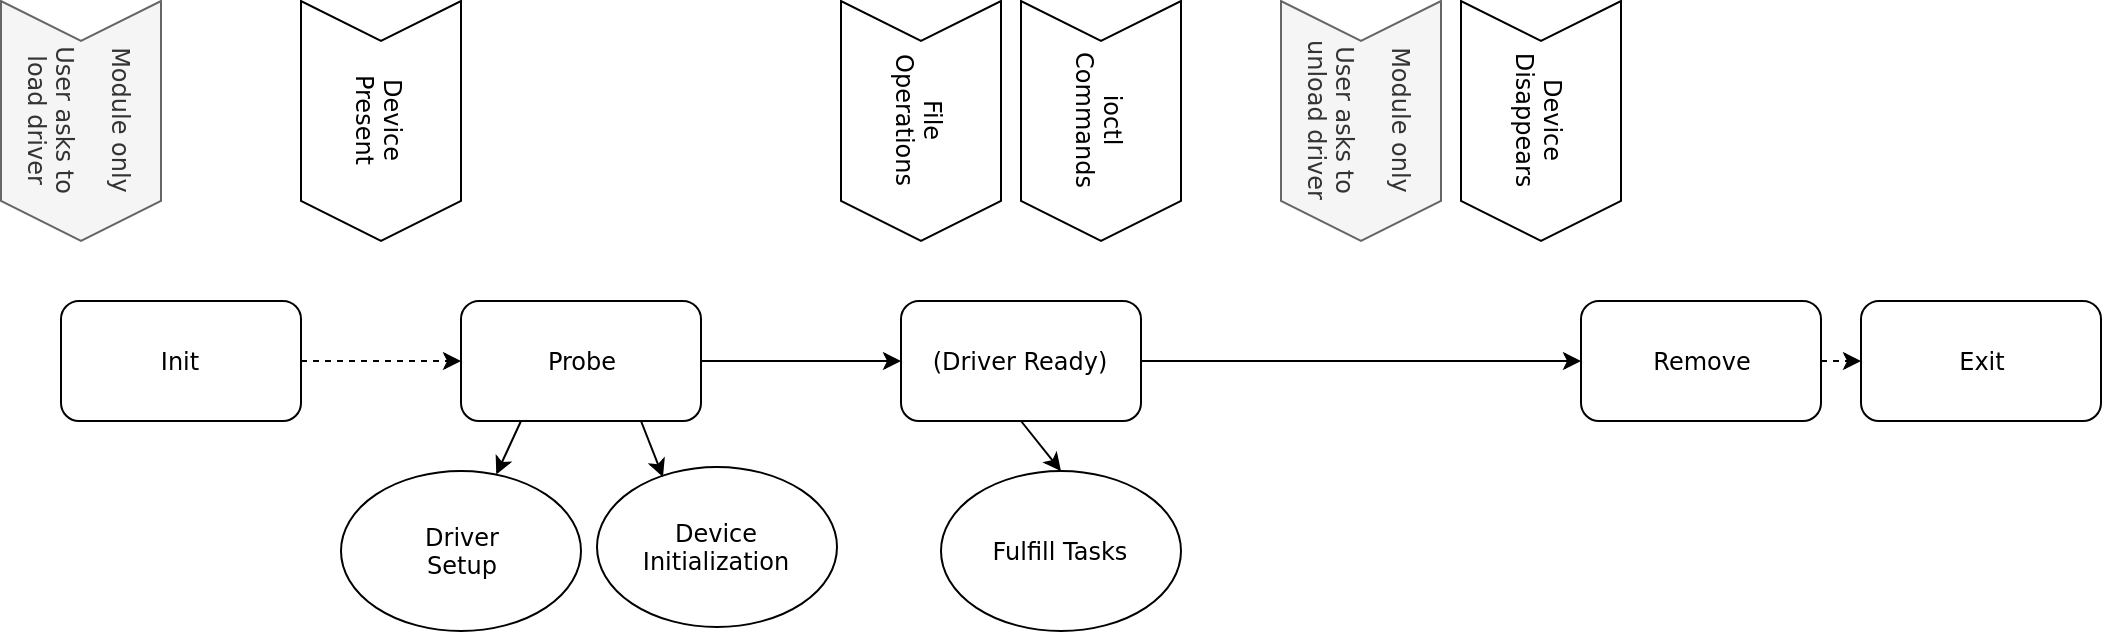
\includegraphics[width=\linewidth]{LinuxDriverLifecycle}
    \caption{Simplified Lifecycle of a Linux Device Driver}
    \label{pic:linux-lifecycle}
\end{figure}
%
%
Only afterwards, the \texttt{exit()} function can be called.
Within \texttt{exit()}, the device should be put in a suitable condition prior to the initialization done in \texttt{probe()} is revoked\cite{lfd430},~\cite{quade2016Linux}.
The \texttt{remove()} function is \textit{re-entrant}, too.
It is called per device.
The right information needed to deregister a device and the driver's entries for this specific instance should be stored as part of the private per-device datastructure.
Figure~\ref{pic:linux-lifecycle} illustrates this situation.

After probing the device, the driver for this instance is ready for use.
Different interfaces to a driver in Linux were already mentioned in a previous section.
Figure~\ref{pic:linux-lifecycle} only pictures the file operations and \texttt{ioctl()} as a special situation within them.
Regardless of the used interface, all corresponding implementations in the driver must be \textit{re-entrant}, but not only in terms of different device instances using the same driver code, but also for a single instance receiving multiple requests, e.g.\ from different users.
The implementations task is decoding the user's request, translating it in a command for the device controller and taking care of the physical transmission to the device.
Depending on the request, this may include sending requests for actions, commands and data to the device but also fetching answers, status codes and e.g.\ processed data from it\cite{quade2016Linux}.


\section{Zircon Driver Model}
The driver model in Zircon differs a lot compared to Linux due to the influences of the microkernel approach.
This concerns in particular mechanisms and corresponding terms which are used by the system to manage device drivers and enable them in userspace.
Nevertheless, a driver in Zircon has the same purpose as a Linux one: providing a uniform interface to a specific device while its implementation details are hidden\cite{zircon-ddk-gettingstarted}. 

\subsubsection*{Device Model}
Zircon's model for devices and drivers is a direct result of choosing a microkernel approach and at the same time a rejection of the situation in Linux.
There, device drivers live in the kernel's address space with privileged access to the whole kernel memory and other resources.
As a result, each part of the kernel including device drivers belong to the same process.
A fault isolation within the Linux kernel is not given and a bad driver may break the entire kernel. 
In contrast, a pure textbook approach for a microkernel would run each single driver in its own process to reach the maximum possible isolation.
Even if some real-world microkernel implementations do so, it is not an efficient approach as it requires a great amount of context switches and \ac{ipc}\cite{zircon-ddk-gettingstarted}.
Thus, Zircon's idea differs from the textbook approach and groups a number of related drivers together in so-called \textit{device host} processes\cite{zircon-ddk-gettingstarted}.
A driver itself in Zircon is compiled to an \acf{elf} shared library, a \ac{dso}.

Another related mechanism in the Zircon kernel is the \textit{device manager process (devmgr)}.
It contains the \textit{device coordinator}, a piece of software that keeps track of drivers and devices.
The device coordinator manages the discovery of drivers and devices and is responsible for the creation of device host processes.
A \ac{dso} driver is loaded into a \textit{device host (devhost)} process and lives there, maybe together with other related drivers, to reduce needed context switches without softening the microkernel concept too much.
In addition, the coordinator maintains the \textit{device filesystem (devfs)} as a mechanism that enables userspace applications to access a driver and thus, the device too.
Similar to the unified device model in Linux, the Zircon device coordinator views devices as a part of a unified tree structure\cite{zircon-devicemodel},~\cite{zircon-ddk-gettingstarted}.
Branches of this tree are represented by device host processes which consist of devices.
In the current state of Zircon, the policy used to decide which drivers are grouped together for performance reasons and which ones should be placed into separate device host processes is made based on the underlying physical system.
As a result, each device that is able to represent a physical bus master becomes a device host process and all corresponding child devices are placed into this process.
In the future, this policy will possibly evolve into a more sophisticated concept\cite{zircon-devicemodel}.

In Zircon, device drivers may implement \textit{protocols}, that means C \acp{abi}.
A protocol is a strict interface definition and defines a set of functions a driver must implement.
Protocols are specific to classes of devices.
As a result, all devices from a type, e.g.\ \ac{pci} devices must implement the same protocol and thus, the same functions.
Zircon differentiates rather in device protocol types such as \textit{\ac{pci}, \ac{usb}, block core or ethermac} than in block, character or network devices.
A protocol is used by child drivers to interact with its parent drivers in a device specific manner.
So it is an interface protocol between different driver layers, and thus commonly different device host processes, for a particular device type or between drivers in the same device host process\cite{zircon-ddk-gettingstarted},~\cite{zircon-devicemodel}.

Additionally, a device can implement \textit{interfaces}.
They represent \textit{\ac{rpc} protocols} which are used by userspace applications or services.
Interfaces are for example the \ac{posix} styled \texttt{open()}, \texttt{close()}, \texttt{read()}, \texttt{write()} or \texttt{ioctl()} functions but also own interfaces defined using the Zircon specific \acf{fidl}\cite{zircon-devicemodel}.

Within the device filesystem (devfs), Zircon devices respectively drivers are grouped in \textit{classes}.
A class represents in this situation a promise to implement certain protocols and/or interfaces.
Devices exist in devfs in a structured way under a topological path according to the scheme \texttt{/dev/class/device/drivername}, e.g.\ \\
\texttt{/dev/pci/00:02:00/intel-ethernet}.
At the time of writing, the names within the class directories, the device identifiers, are unique numbers in a certain pattern\cite{zircon-devicemodel}.
%TODO -> check classes in runnin zircon

% %General
    % \cite{zircon-ddk-gettingstarted}
    % - zircon: use concept of device host
        % - devhost is a process that contains a protocol stack (one or more protocols that work together)
        % -> devhost loads drivers from elf shared libraries (dsos)
        % -> the protocol stack allows the creation of a complete ``driver'' for a device, consisting of platform dependent and platform independent components -> self contained process container
%
\subsubsection*{Driver Lifecycle}\label{sec:zirconlifecycle}
It is currently not possible in Zircon to built drivers in a different way than the built-in \textit{\ac{elf} shared libraries} mentioned before.
They are not loaded into a device host process until it is determined they are actually needed.
This is done using the \textit{binding program} which is a part of the driver.
Within the driver, it is defined using system internal macros.
The compiler moves this program into the \textit{ELF NOTE} section of the binary where it can be inspected by the \textit{device coordinator} without the need to fully load the driver into its own process.
Besides the bind description itself, the binding program also contains pointers to the most important driver methods\cite{zircon-devicemodel}.

The first but less used method in the Zircon device driver lifecycle is \texttt{init()}.
It is invoked when a driver is loaded into a device host process and used for any global initialization.
While its equivalent in Linux is often replaced using macros to reduce boilerplate code, Zircon makes it optional to implement it.
Typically, no implementation for \texttt{init()} is required but if the method is implemented and fails, the whole driver fails\cite{zircon-devicemodel}.
It is pictured in the simplified Zircon driver lifecycle as an optional operation in figure~\ref{pic:zircon-lifecycle}.

Similar to Linux' \texttt{probe()} function follows in Zircon the \texttt{bind()} method in a driver's life.
It is invoked by the device coordinator which offers the driver a device to bind.
This device matches the rules the driver has published as a part of its bind program.
Within \texttt{bind()}, the driver has to initialize the device, setup interfaces to itself and publish one or more childs of the device to succeed\cite{zircon-ddk-gettingstarted}.
Adding such a child device is done using \texttt{device\_add()}.
It creates a new device and adds it as a child to a provided parent device.
This parent must either be exactly the device which is passed to \texttt{bind()} by the device coordinator or another device which already has been created by the same device driver.
This method includes adding the newly created device to the device filesystem (devfs) which is maintained by the device coordinator.
As soon as a device is added to devfs, the device operations, e.g. \texttt{read()}, \texttt{write()} or calls defined using \ac{fidl}, can be called by the device host.
Figure~\ref{pic:zircon-lifecycle} illustrates the simplified situation.
If a device shall be added but not be accessed already, e.g.\ to do a longer initialization as a background thread, the device can also be added in an invisible mode using a specific flag.
After the initialization is done, the device must be made visible to be accessed\cite{zircon-devicemodel}.

The device driver method \texttt{create()} is only invoked for platform or system bus drivers or proxy drivers.
Thus, it concerns only very few drivers and is not further considered in this work or the related figure\cite{zircon-devicemodel}.
%
\begin{figure} [t]
    \centering
    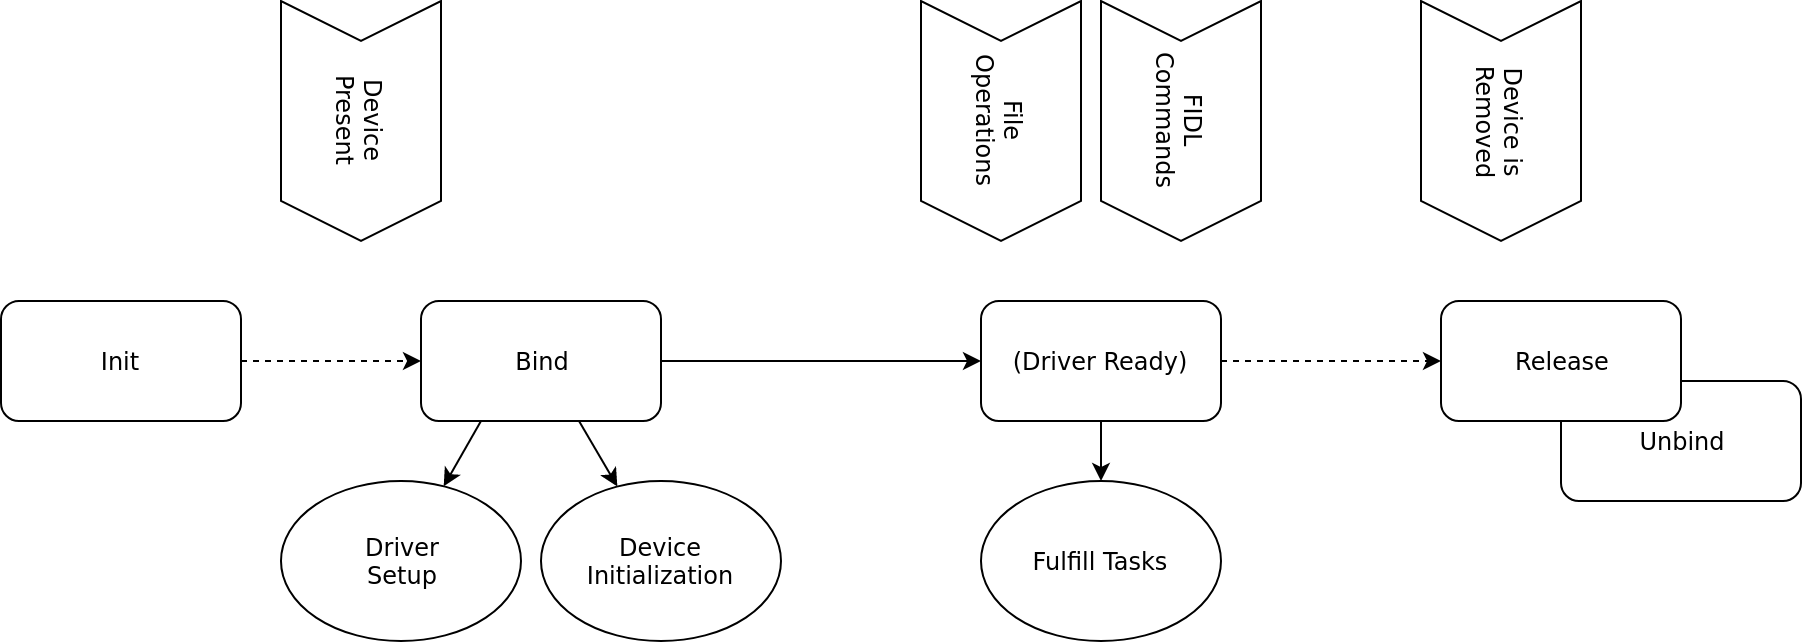
\includegraphics[width=\linewidth]{ZirconDriverLifecycle}
    \caption{Simplified Lifecycle of a Zircon Device Driver}
    \label{pic:zircon-lifecycle}
\end{figure}
%
The driver's \texttt{release()} method is invoked right before the driver is unloaded and after all devices it may have created in \texttt{bind()} using \texttt{device\_add()} have been destroyed.
The method is currently never invoked because once a driver is loaded, it remains loaded for the lifetime of a device host process.
Nevertheless, it should be implemented.

In theory, \texttt{release()} and the related \texttt{unbind()} method should be called e.g.\ if a parent device detects the corresponding device is removed and thus, calls \texttt{device\_remove()} as pictured in figure~\ref{pic:zircon-lifecycle}.
In consequence, the \texttt{unbind()} method is called on all child devices because the parent becomes removed.
Unbind should remove all interfaces that were created in relation to the \texttt{device\_add()} call.
If a device still has work in progress when \texttt{unbind()} is called by the parent, the child device continues this first.
Thus, the parent must ensure the device is not working anymore before it also calls \texttt{release()} as a last step in this exemplary tear down sequence on all children\cite{zircon-devicemodel}.


\section{Development Setup}
\subsection{Hardware Selection}
The hardware selection for the driver development case study is limited by the available development platforms for Zircon.
The best known x86\_64 platform is probably Google's own hardware, the \textit{Pixelbook}, which is currently shipped with \textit{Chrome OS}.
Unfortunately, there is hardly anything known about suitable internal hardware for a manageable test driver for e.g.\ sensors.

Thus, the decision was made for an ARM64 based development board with an accessible expansion interface.
The chosen \textbf{HiKey960} is pictured in figure~\ref{pic:hikey}.
It is not only a development board for Linux but also officially listed as reference platform for Google's \textit{Android} operating system.
The HiKey is, amongst other things, equipped with\footnote{96boards.org, visited on 02.05.2019~\url{https://www.96boards.org/product/hikey960/}}
\begin{itemize}
    \item 4 ARM Cortex A73 and 4 ARM Cortex A53 \ac{cpu} cores arranged in the big.LITTLE architecture,
    \item a ARM Mali G71 MP8 \ac{gpu},
    \item 3 GB \ac{ram},
    \item 32 GB Flash Storage,
    \item an expansion interface, in particular consisting of
        \begin{itemize}
            \item UART,
            \item \ac{i2c},
            \item SPI and
            \item GPIO.
        \end{itemize}
\end{itemize}

\begin{figure} [t]
    \centering
    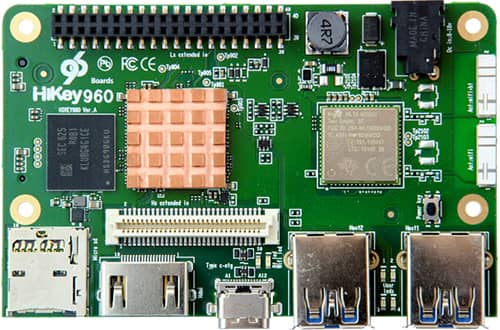
\includegraphics[scale=0.6]{hikey-960-SD-front}
    \caption{HiKey960}\label{pic:hikey}
\end{figure}

The peripheral device for which the driver is written, should provide a well-known interface that is already supported within the Zircon kernel.
\ac{i2c} matches this requirement and driver examples for C and C++ are available in the used Zircon source version.
Of course, \ac{i2c} support is available in Linux, too.
As \ac{i2c} is a very common hardware communication interface manifold devices equipped with this interface are available.
Different sensor types are conceivable as well as actors like displays which is another argument for the decision to use \ac{i2c}.
To make the driver development more sophisticated, the \textbf{Grove-LCD RGB Backlight} peripheral device (see figure~\ref{pic:grove}) was selected.
The peculiar fact about the device is that the \ac{lcd} and the \acs{rgb} backlight are controlled by distinct controllers on the peripheral device.
Using \ac{i2c} enables this situation.
It is a two wired master-slave bus working in a serial transfer mode.
Several masters and slaves are allowed, but both roles can also be combined in one.
A data transfer is initialized by a master reaching out for the desired slave using an address.
For the Grove device, there are two distinct slaves with individual addresses which need to be controlled.
A device's \ac{i2c} address is usually set by the manufacturer but configurable to avoid conflicts on the bus.
For the Grove device, the default slave addresses are \texttt{0x62} for controlling \ac{rgb} and \texttt{0x3e} for LCD\@.
Two additional addresses are available on the combined device, but they are used on startup and can not be addressed individually\footnote{wiki.seeedstudio.com, visited on 15.06.2019 \url{http://wiki.seeedstudio.com/Grove-LCD_RGB_Backlight/}}.
Thus, they do not matter for the driver development.

\begin{figure} [t]
    \centering
    \includegraphics[scale=0.35]{GroveLCD}
    \caption{The Grove-LCD RGB backlight peripheral device}\label{pic:grove}
\end{figure} 

\subsubsection*{Hardware Issues}
The HiKey960 works internally on +1.8V  while the Grove-LCD RGB peripheral device is on +5V.
As a result of not working at the same voltage level adjustments are needed.
Unfortunately, common level shifters did not work in this situation, because the level ranges for detecting a logical \textit{0} respectively for a logical \textit{1} on the Grove differs between both \ac{i2c} controllers.
Thus, a sophisticated level adjustment to match both ranges was needed to solve this issue.
The final resulting circuit is pictured in figure~\ref{pic:groveadjust}.

The practical part of this thesis was started with the development of the Zircon driver.
Thus, the adjusting circuit was in particular designed for exactly one HiKey960 development board.
This board was equipped with the necessary firmware to flash and boot Zircon while two other HiKey960 boards were prepared for booting Linux.
After switching to Linux development and thus to another HiKey960, there were again issues with level adjustment which were expressed by an unreliable or not at all working LCD while the signals on the \ac{i2c} bus captured by an oscilloscope were fine.
The error search indicated that the output levels for \ac{i2c} at all tree available HiKey960 development boards differ in the range of 0.5V.
Accordingly, the two HiKey boards running Linux did not get proper levels to detect a logical \textit{0} respectively a \textit{1} depending on the direction of the deviation.
As an adjustment for another board would have resulted in unreliableness on the Zircon side, the decision was made to port the already existing Linux driver to the Raspberry Pi development board (version 2 or 3).
It is running on +5V per default which makes any level adjustment obsolete. 
A dynamic switching between Zircon and Linux on the exact same HiKey960 board was not possible.
The diverging firmware needed to boot either Zircon or Linux was too error-prone in the setup.
Likewise, a complete change to the Raspberry Pi as a development platform was not possible, since Zircon does not support the board (anymore\footnote{\url{https://github.com/Allegra42/zircon/commit/5dc89c3f67808804c0c7d1bd9a0df3703d961ce6#diff-9bd3cb9d38dba050f310f03d18bbb2cf}}).
The final setups used for Zircon driver development and the remaining Linux development are pictured in figure~\ref{pic:zirconsetup} (Zircon) and figure~\ref{pic:linuxsetup} (Linux).
This change does not influence the driver development in any manner.

\begin{figure} [t]
    \centering
    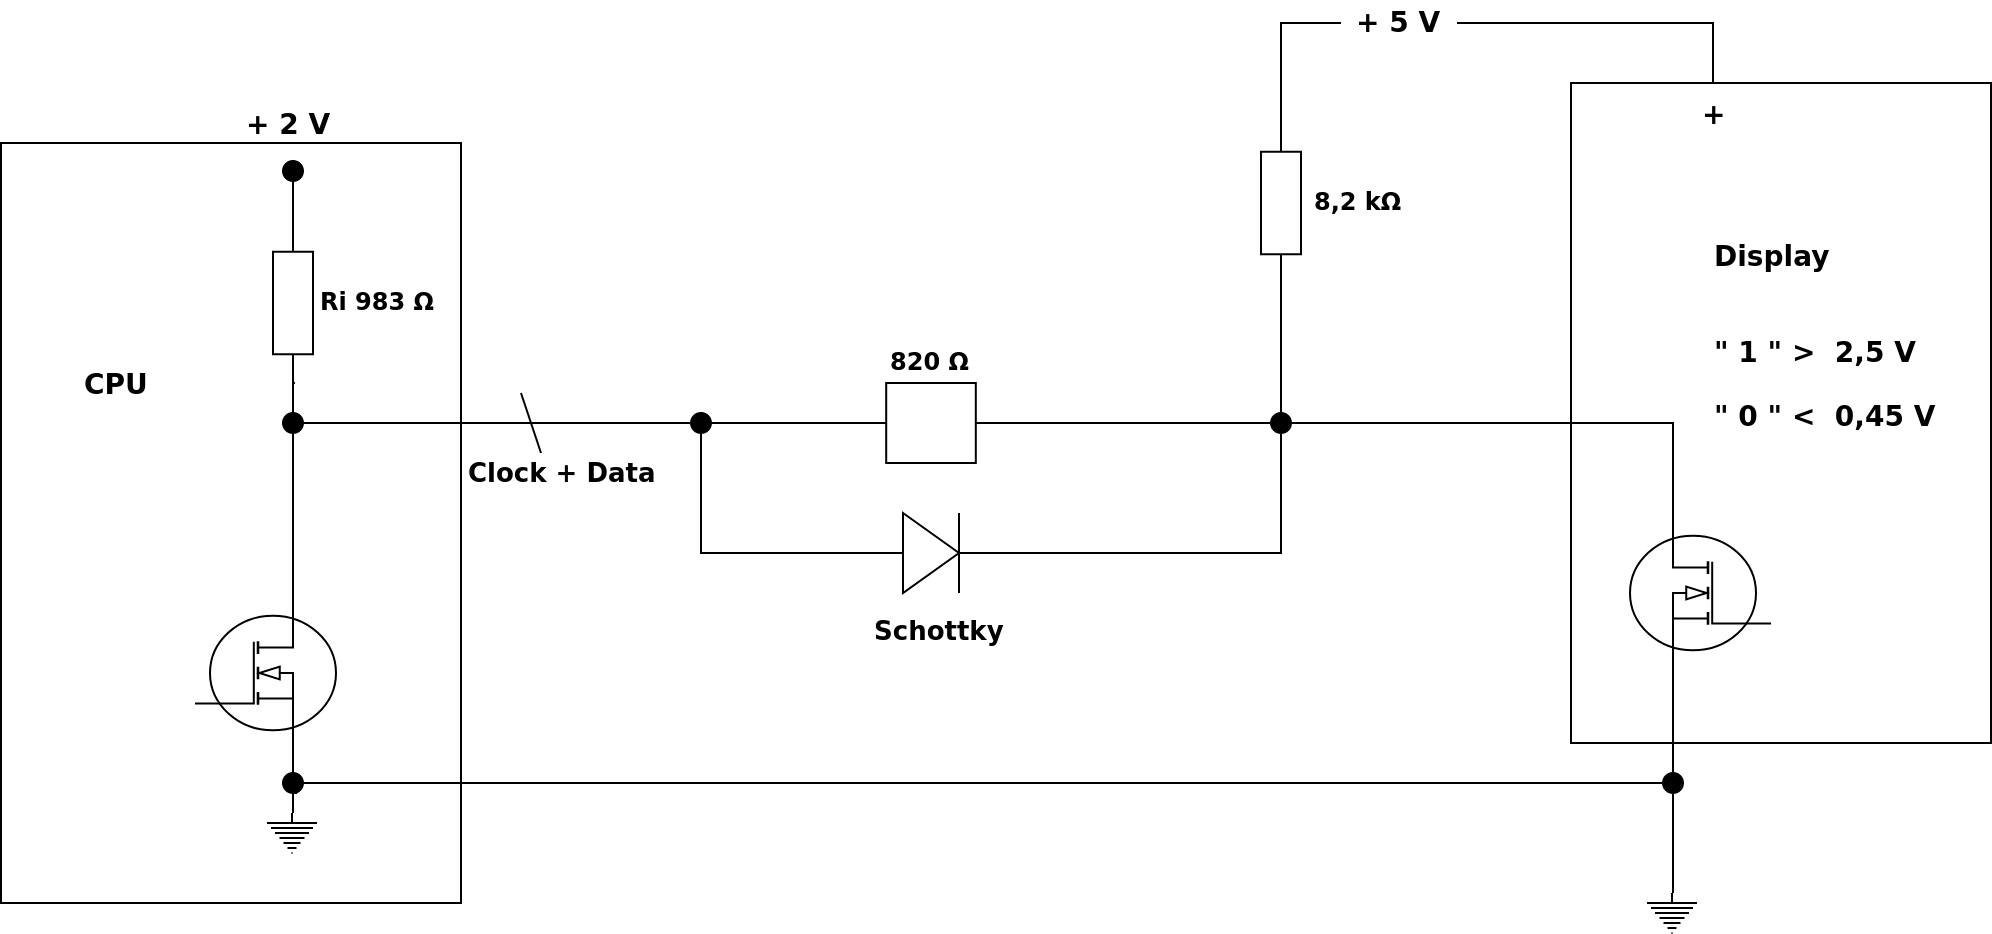
\includegraphics[width=\linewidth]{GroveAdjustment}
    \caption{Level Adjustment for the Grove RGB LCD with the HiKey960 Development Board}\label{pic:groveadjust}
\end{figure} 

\begin{figure} [H]
    \centering
    \includegraphics[scale=0.3]{ZirconSetup2}
    \caption{Final Development Setup for Zircon using the HiKey960 Development Board}\label{pic:zirconsetup}
\end{figure} 

\begin{figure} [ht]
    \centering
    \includegraphics[scale=0.35]{LinuxSetup}
    \caption{Final Development Setup for Linux using the Raspberry Pi Development Board}\label{pic:linuxsetup}
\end{figure} 


\subsection{Software Development Setup}
\subsubsection*{Linux}
Initially, the Linux driver development was based on a mainline kernel in version 4.9.
Due to the needed platform change, the already existing driver was ported to the Raspberry Pi Linux kernel tree in version 5.0.
For a stable source code base over this thesis' duration, the kernel's source repository was forked and all development done in a branch of the fork.
The repository is publicly accessible on GitHub\footnote{\url{https://github.com/Allegra42/linux-rpi}}.

The Raspberry Pi runs a standard Raspbian Linux, just the kernel respectively the driver module need to be changed during development.
Corresponding scripts to build kernel and modules for a Raspberry 2 or 3 running Raspbian and flash the binaries to a prepared SD card are part of the repository, too.
By switching to the specific Linux kernel tree for the Raspberry Pi, there is no default support for using \textbf{Clang} as compiler anymore.
Some device specific changes in this kernel tree impede the Clang build and would need manual adjustments.
The use of Clang related tools, especially \textit{ClangFormat} is not affected.

Within this work, the Raspberry Pi runs without an attached display besides the Grove-LCD RGB peripheral.
The development board is accessed using its physical \ac{uart} interface with a \ac{usb} to serial \ac{ttl} adapter which allows the connection to a terminal session.


\subsubsection*{Zircon}
The Zircon kernel consists of the actual kernel, a bootloader, system modules, third-party modules and scripts.
\textit{System modules} include necessary system facilities like the already mentioned device manager, but also the effective device drivers, or system-relevant user applications.
Zircon is not built in versioned releases, yet.
To work on a stable code base, nevertheless, the Zircon repository on GitHub was forked in December 2018.
Today, due to restructurings from Google, the origin repository is no longer available and even the standalone Zircon code moved into the Fuchsia source tree on GoogleSource\footnote{\url{https://fuchsia.googlesource.com/fuchsia/+/refs/heads/master/zircon/}}.
Accordingly, the driver development but also this work in general refer to the forked Zircon source tree\footnote{\url{https://github.com/Allegra42/zircon}}.

In contrast to Linux, Zircon is booted as a standalone system for this thesis.
The Fuchsia userland is not used at all.
Thus, the tooling of the running kernel is limited and just a subset of the console commands and interactions known from Linux or Fuchsia is available.
This concerns i.a.\ the Unix-like tool \texttt{cat} which is, for example, used to read from device files, while \texttt{echo}, which is used to write into device files, is available.
As an alternative option, an implementation of the older Unix tool \texttt{dd} can be used within the pure Zircon kernel.

For the development of Zircon including drivers and operating system related\\userspace modules both compilers, GCC and Clang, are available.
While GCC is default in most situations and scripts, e.g.\ in the built script for the HiKey960 which is a native part of the source tree, the surrounding tools like code formatting or linter are clearly based on Clang and may require a Clang build to work.

Just like Linux, the Zircon development setup is accessed via its \ac{uart} interface.
The setup is the same as for Linux, no matter whether using a Raspberry Pi or the HiKey960.
Without Fuchsia as an userland, Zircon is not running a full graphics stack at all and thus, would not be able to show a \ac{gui} in contrast to Linux respectively Raspbian.
As the HiKey960 is not equipped with a physical ethernet interface, \ac{uart} is the only way to interact with Zircon.
% For both, Linux and Zircon, the \ac{uart} also shows kernel messages.

  
\section{General Driver Concept}\label{sec:cs-driver-concept}
In general, the driver concept for both, Linux and Zircon should be very similar because the Grove-LCD RGB backlight as peripheral device specifies them and stays the same on both platforms.
However, both operating system kernels add some requirements, too.

Nevertheless, the first decision for the driver concept is caused by the Grove-LCD RGB backlight's nature of combining two distinct device controllers into a single peripheral device.
Especially in Linux, two distinct \ac{i2c} devices, i.e.\ two controllers and thus two slave addresses, required distinct device drivers until kernel 4.9.
Only later Linux kernel versions allow a combined driver from two or more related \ac{i2c} slave addresses by providing an appropriate \ac{api}.
Zircon also allows combined \ac{i2c} drivers in the used version level, but only on so-called \textit{platform devices}.
The corresponding term \textit{platform bus} describes the Zircon driver for a framework that manages several low level drivers on ARM64 system architectures.
An \ac{i2c} driver is in this context a \textit{protocol implementation driver} and thus a part of the \textit{platform bus}.
Such a driver is running in the same device host as the bus driver itself\cite{zircon-platformbus}.
The situation is illustrated in figure~\ref{pic:platformbus} which is also a part of the official Zircon documentation\footnote{\url{https://github.com/Allegra42/zircon/blob/i2c-grove-lcd/docs/ddk/platform-bus.png}}\cite{zircon-platformbus}.

\begin{figure} [t]
    \centering
    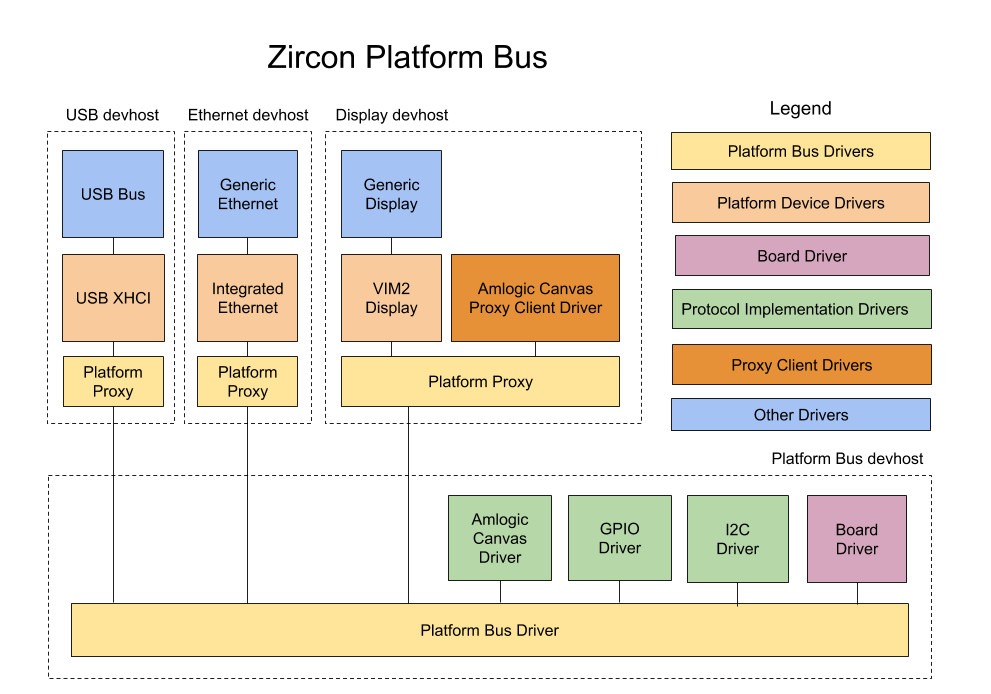
\includegraphics[scale=0.35]{platform-bus}
    \caption{The setup of the Zircon Platform Bus on ARM64 based devices\cite{zircon-platformbus}}\label{pic:platformbus}
\end{figure} 

However, the possibility to write a combined driver for both parts of the Grove is right now exclusively limited to platform devices.
Indeed, the development setup using the HiKey960 and the Grove-LCD RGB backlight device fulfills this requirement but in contrast to Linux the needed \ac{api} is not fully available.

For this work, the decision was made to use the new \ac{api} for a combined driver on Linux.
It is still new and rarely used right now but interesting, globally available but above all, it is more meaningful for devices which are consisting from more than one \ac{i2c} controllers, such as the Grove RGB LCD backlight device.
Perspectively, it is to be expected that more similar device driver implementations will switch to this \ac{api}.
One positive consequence of switching is the need of less boilerplate code.
For example it is not longer needed to write two or more pretty similar initialization routines for each partial driver.
In the device filesystem \texttt{/dev/}, the Grove peripheral also shows up as a single device which corresponds more closely to reality than distinct part devices.
A further consequence of this decision results for an user's access to the driver.
The standard file operations \texttt{read()} and \texttt{write()} are no longer meaningful for the device.
Using distinct drivers, especially for the \ac{lcd}, both of them are meaningful and thus useful, but already the meaning for the \ac{rgb} part is more complicated.
While it is very clear that a string which is sent to a line display should be shown, to a \ac{rgb} backlight device is not that meaningful.
It requires a certain non-intuitive format to be understood.
By implementing distinct drivers, this is to some degree possible without losing meaning and the intuitive nature of especially the \texttt{write()} call, but a combined driver would imply a sophisticated string parsing to differentiate between both devices.
Thus, the usage of \texttt{write()} would not be intuitive for users anymore.
As a result, implementing those calls does not make sense for this kind of driver.
Instead, \texttt{ioctl()} commands or specifically defined pseudo-files in sysfs or procfs are a more conceivable solution for the Linux driver.

In Zircon, the situation is very similar to Linux.
But the \ac{api} for a combined driver is not available on x86\_64 platforms.
Using the combined \textit{platform device \ac{api}}, implementation standard file operations are, like in the Linux case, not meaningful.
Besides, the way file operations are implemented in Zircon is not considered as known as it is for Linux.
Thus, both variants, the two driver versions which are also usable on x86\_64, but also the platform device way, are interesting for this work and should be considered.
Using the HiKey960 as a hardware platform enables both.
While the standard file operations are available on both, Linux and Zircon, the further interfaces differ between them.
Zircon offers with a \ac{fidl} defined \acs{api} a very sophisticated option for driver specific interfaces which is comparable to the also available \ac{io}-controls but there are not equivalents to sysfs or procfs.
To keep the drivers on both systems comparable and limit the development effort, they are not further considered in this work.
Of course, even more comparable would be the use of \texttt{ioctl()} on both operating systems, but this would break the idea of writing idiomatic code for both platforms.
According to the documentation are interface definitions using \ac{fidl} clearly preferred in Zircon\cite{zircon-ddk-gettingstarted}.
Although the trend in Linux goes away from \texttt{ioctl()} to implement meaningful virtual file entries for sysfs the former ones are still accepted and wide-spread while Zircon clearly prefers the use of \ac{fidl} in such a situation.
Furthermore, the virtual entries below a sysfs record are hardly comparable to \ac{io}-controls or \ac{fidl} in terms of defining type-safe call signatures with several arguments and types.

Additionally, Zircon enables driver development in different languages.
For the source code version used within this work, these are \textit{C} and \textit{C++}.
Using C as a programming language for drivers implies good documentation and lot of examples within the code.
C++ is less documented in the used version but also in Google's master repository.
Nevertheless, documentation and code are clearly in favor of C++ drivers and more and more C drivers are moved to C++.
Accordingly, both ways are very attractive for this work, C++ in particular as drivers in this language are a great difference to Linux ones.

The chosen compiler does not influence the actual driver development to a major degree, but it does for the system.
Most of all, the error messages, diagnostics and some internal details are the obvious parts that may differ between GCC and Clang.
They may also influence the output, but syntax errors are found on both of them.
Hence, the possibility to compare two builds from different compilers is at all very useful, e.g.\ in cases of compiler errors, but also to compare code sizes, binary or build performances or code portability.
On Zircon, Clang is slightly preferred as a respective build is needed for surrounding tools while GCC is often default for build scripts.
GCC, on the other hand, was very closely interlocked with Linux for a long time.
But also in this case, the opportunity to compare the outputs of two compilers is helpful and the work that was done to decouple Linux and GCC to enable Clang is a positive one.
Another reason for the use of Clang in Linux is, like for Zircon, the surrounding tools e.g.\ for style checking, linting, static and dynamic code analysis or address sanitizing\cite{linux-llvm}.
However, without a closer look into the generated binaries a well-founded choice of the compiler for the pure driver development is rather difficult.
Due to the change to the Raspberry Pi as a hardware platform for Linux driver development, Clang can not longer be used out of the box for compilation but before this change, both compilers and resulting kernels were used.
The same is and may should still be done for Zircon, e.g.\ to see changes in the tooling of both compilers.

%TODO functional scope
The last but important issue for a general driver concept is the question of the implemented functional scope.
The Grove-LCD RGB backlight as a peripheral device is rather complex, not only because of its two controllers.
It is also on account of its LCD controller and its complex and detailed internal instruction set.
Already the Arduino library provided from the manufacturer for this device defines about 14 LCD methods.
Implementing all of them as a part of the drivers in all Linux and Zircon variants with meaningful user interfaces would go beyond the scope of this work without adding a value.
Thus, all drivers should implement the same basic functionality to show general driver concepts.
Because of the decision to write only a combined driver in Linux, this variant lacks support for \texttt{read()} and \texttt{write()} but the additional defined interfacing options for the user, i.e.\ \texttt{ioctl()} for Linux and \textit{FIDL} for Zircon, stay the same.
As a result, the Zircon \textit{platform device} drivers represent the same functionality as the Linux driver.
Respectively, a combined driver should provide in each case a way to:
\begin{itemize}
    \item set the backlight color,
    \item get the backlight color,
    \item clear the shown text on the LCD,
    \item write the first LCD line,
    \item write the second LCD line,
    \item read the whole LCD content and
    \item get the size of a LCD line.
\end{itemize}
The function arguments for these operations should be the same on both operating systems as far as it is permitted by the used interface mechanism.
With these selected functions, the driver implementations should cover the exchange of the most important data types between user and kernel space in both directions.
Not depicted is e.g.\ memory mapping or \ac{dma} as there is no meaningful implementation for the device.

The variants using two distinct driver implementations provide exactly the same functionality respectively the same interface definition but divided between both controllers.
Thus, the first two named requirements belong to the RGB driver while the remaining ones are part of the LCD driver.
Additionally, these driver types should implement \texttt{read()} and \texttt{write()}.
On the LCD side, they should write the user's input to the device file at the LCD's first line for \texttt{write()} and read the entire content of the LCD for \texttt{read()}.
Hence, their implementation is very similar to the explicitly defined device operations above.
In Linux, this would mean the implementation of e.g.\ writing the first line as a part of \texttt{ioctl()} would not differentiate more profoundly from the one for \texttt{write()}.
Only the function signature and thus the copying of data between user and kernel would be slightly different but not the general file operation specific issues in Linux, the used helper functions and the actual invocation of the peripheral.
This does not justify the development of a whole second driver variant in Linux, but the differences in these functions should be mentioned as a part of this work, nevertheless.
These methods are more interesting for this work, especially in the Zircon C++ implementation.


\section{Linux Driver Development}\label{sec:cs-linux}

  \subsection{Prearrangements}\label{sec:linux:prearrangements}
To build a Linux driver, various options are available.
It can be built as a permanent part of the kernel as a \textit{built-in} driver or as a \textit{module}.
% Further, it is not needed a module's source code is located within the actual kernel source tree.
For this work, the first choice should not play a major role, but the source location.
Carefully developed as a module within the kernel sources, the change to \textit{built-in} is nothing more than a build configuration.
Accordingly, the driver must be placed into the internal kernel structure in a meaningful manner.
Linux is organized into \textit{subsystems} to structure its monolithic architecture into functionally related modules.
Within the \textit{drivers} directory, there are several subsystems which are more or less meaningful for the Grove display.
The probably most appropriate subsystem for this device is \textit{auxdisplay}, i.e.\ auxiliary display which groups a small amount of drivers for small additional displays e.g.\ \ac{lcd}'s.
Currently, the auxdisplay subsystem consists of only nine drivers.
Each one is made from a single C code file and thus, not further divided into sub-directories for the drivers.
The Grove driver must be to be inserted in this structure.
Therefore, the driver source file is placed in \texttt{drivers/auxdisplay} and its build rules are added in the general \texttt{Makefile} for this subsystem.
To configure the build, i.e.\ if the driver should be built as part of the kernel or as a module or none at all, it must also be registered in the subsystems \texttt{Kconfig} file.
Listing~\ref{lst:make} shows both entries in a combined view.
The actual configuration is done via device specific configuration files, e.g.\ \mintinline{bash}{arch/arm/configs/bcm2709_defconfig}.
Mostly, these long files are not directly modified.
Instead, the command \mintinline{bash}{make menuconfig} is used as a front-end.
It parses the \mintinline{bash}{Kconfig} files within the whole kernel and represents them in their tree structure.
The Grove driver for example, is part of the \mintinline{bash}{auxdisplay} subsystem.
Thus, general support for auxdisplays must be enabled to build also the Grove driver.
%
\begin{listing} [ht]
\caption{Build Configuration for the Grove-LCD RGB backlight driver}
\label{lst:make}
\begin{minted}[frame=lines, framesep=2mm, fontsize=\footnotesize, linenos, breaklines]{make}
# Make Entry
obj-$(CONFIG_GROVE)			+= grove.o

# Kconfig Entry
config GROVE
tristate "Grove-LCD RGB backlight v4.0 Support"
default m
---help---
    Enable support for the Grove-LCD RGB backlight v4.0 via I2C.
    The device is accessible via "/dev/grove" char device.
    For the interface see "include/uapi/linux/grove_ioctl.h".
\end{minted}
\end{listing}
%
The help text shown for the driver configuration shown in listing~\ref{lst:make} mentions the path \texttt{include/uapi/linux/grove\_ioctl.h}.
It contains the custom \texttt{ioctl()} call definitions.
They should be accessible from both, kernel and userspace.
Thus, the definition for this and other drivers are collected under this path.

The Linux driver discussed in this section is a complex software implementation.
Even if its nature, consisting of two distinct device controllers, make the development more interesting, it is neither necessary nor possible to talk about the device specific implementation in all details within this work.
Thus, only specific code snippets are discussed.
The full Linux driver source code is available at \url{https://github.com/Allegra42/linux-rpi/blob/rpi-5.0.y/drivers/auxdisplay/grove.c}.

\subsection{Driver Initialization and Exit}
For the Grove driver, there is no need for additional one time initialization that is commonly done within the regular \mintinline{c}{module_init()} call.
As already mentioned, the Linux kernel provides macros instead to register the driver without unnecessary boilerplate code.
For an \ac{i2c} driver as the Grove is, the matching macro is \mintinline{c}{module_i2c_driver()} (see listing~\ref{lst:init}, line 17).
It takes an \mintinline{c}{i2c_driver} structure (see listing~\ref{lst:init}, line 8) as an argument which contains function pointers to the driver implementation of \mintinline{c}{probe()} and \mintinline{c}{remove()}, but also driver specific information like its name and a further pointer to an \mintinline{c}{of_device_id} table.
This table defines a set of properties, e.g.\ so-called \textit{compatible strings} (listing~\ref{lst:init}, line 2).
As the Raspberry Pi is an ARM architecture, its actual hardware configuration and thus also firmly attached devices like the Grove are defined in a specific file, the \textit{device tree}. 
%
\begin{listing} [ht]
    \caption{Driver Initialization Sequence using \texttt{module\_i2c\_driver()}}
    \label{lst:init}
    \begin{minted}[frame=lines, framesep=2mm, fontsize=\footnotesize, linenos, breaklines]{c}
static const struct of_device_id grove_of_idtable[] = {
    { .compatible = "grove,lcd" },
    {}
};

MODULE_DEVICE_TABLE(of, grove_of_idtable);

static struct i2c_driver grove_driver = {
    .driver = {
        .name = "grove",
        .of_match_table = grove_of_idtable
    },
    .probe_new = grove_probe,
    .remove = grove_remove,
};
%
module_i2c_driver(grove_driver);
    \end{minted}
\end{listing}
%
Within the device tree, an entry which defines the relevant information about the Grove-LCD RGB backlight device is needed.
Listing~\ref{lst:devtree} shows this definition.
From the system's view, this information is the superior \ac{i2c} node the device is attached to and the device's addresses on the bus.
%
\begin{listing} [ht]
    \caption{Device Tree Configuration for the Grove Peripheral Device}
    \label{lst:devtree}
    \begin{minted}[frame=lines, framesep=2mm, fontsize=\footnotesize, linenos, breaklines]{c}
&i2c1 {
  pinctrl-names = "default";
  pinctrl-0 = <&i2c1_pins>;
  clock-frequency = <100000>;
  grovei2c: grove-i2c@3e {
    compatible = "grove,lcd";
    reg = <0x3e 0x62>;
    reg-names = "grovelcd", "grovergb";
  };
};
    \end{minted}
\end{listing}
%
Besides, for the matching between the actual device and the driver the \textit{compatible string} is a crucial information.
It is defined according to a defined scheme of the manufacturer and the device name (see listing~\ref{lst:devtree}, line 6).
To take advantage from the new Linux \ac{api} which enables a single driver for combined \ac{i2c} devices from two or more bus slaves, their addresses and subnames must be defined in a specific manner shown in listing~\ref{lst:devtree}, line 7 and 8.
Defining, in this case, both partial \ac{i2c} devices within an own node would not work in the context of this \ac{api}.
Unfortunately, this special requirement is rarely documented right now, maybe because the use of this feature within the mainline kernel is still very limited.

To come back to the tasks of \mintinline{c}{module_i2c_driver()}, the focus returns to the way a module is registered in the system.
Thus, the function pointers in listing~\ref{lst:init} line 12 and 13 are also decisive.
The structure given to \mintinline{c}{module_i2c_driver()} contains, besides the matching related entries, function pointers to the driver's implementations for \mintinline{c}{probe()} and \mintinline{c}{release()}.
After registering the driver by the system using this structure and the macro, exactly this driver's \mintinline{c}{probe()} is called for a device with a matching compatible string.
Indeed, the device tree used for ARM architectures is at first a static structure, but it can be extended at runtime using \textit{device tree overlays} which provide a kind of \textit{hotplugging} for device types like \ac{i2c} on ARM.
The last and unusual issue in listing~\ref{lst:init} is the structure's entry for the \mintinline{c}{probe()} function in line 13.
It is \mintinline{c}{probe_new()} instead of \mintinline{c}{probe()}, but the reason for this is simple.
The current function signature for probing an \ac{i2c} device will change in the future and \mintinline{c}{probe_new()} already takes a function pointer to the new one.
As there is no need for the now deprecated one within this driver, the new function signature should be used.

Using the \mintinline{c}{module_i2c_driver()} macro also means \mintinline{c}{exit()} does nothing special and thus, it is not further mentioned.

\subsection{Device Probing and Releasing}
As already discussed, the \mintinline{c}{probe()} implementation in listing~\ref{lst:probe} already uses the new method signature.
The previously used second argument, the\\\mintinline{c}{struct i2c_device_id *id}, is not needed for this driver.
As shown in figure~\ref{pic:linux-lifecycle} the driver's implementation of probe is roughly divisible into two parts: the driver's own setup including its registration within the system and the device specific initialization.
The first part is very similar for many drivers.
It includes i.a.\ allocating private memory regions and device numbers but also creating entries in sysfs and devfs.
Often, a driver supports a few similar devices or device revisions which differ in their needs e.g.\ for setting them up or their instruction set.
In such a case, the driver must check within \mintinline{c}{probe()} if the probed device is actually a supported one and how it must be handled.
The grove driver only allows a single compatible string.
A decision between two similar devices is not needed within this work.
The whole setup is under control, a similar device which would require a distinction will not be added.
Also, an additional testing if the device matches is redundant as long as the driver fails if the addresses defined within the device tree are not detected on the bus or the specific initialization failed.

The \mintinline{c}{probe()} function is the first function of this driver which must be \textit{re-entrant} and aware of more than one device to handle.
Thus, a structure for device specific and private data is needed.
It is globally defined within this driver and should contain the needed information to restore a device and its state from each possible driver entry point.
For the Grove peripheral, it is e.g.\ 
\begin{itemize}
    \item the device number \mintinline{c}{dev_t devnum}, which merges \textit{major} and \textit{minor} numbers,
    \item the character device \mintinline{c}{struct cdev cdev},
    \item pointers to the \ac{i2c} device instances \mintinline{c}{struct i2c_client *client} for both, \ac{rgb} and \ac{lcd} and 
    \item device specific private data to restore the device's state, i.e.\ a struct to store color information and char buffers for the \ac{lcd} content.
\end{itemize}
The reasons for storing exactly these information within the struct defined as\\\mintinline{c}{struct grove_t} become clear in the course of this driver's analysis.

\begin{listing} [H]
    \caption{Device Probing}
    \label{lst:probe}
    \begin{minted}[frame=lines, framesep=2mm, fontsize=\footnotesize, linenos, breaklines]{c}
static int grove_probe(struct i2c_client *client)
{
  int ret = 0;
  struct grove_t *grove;
  struct device *dev = &client->dev;  // Store I2C client device
  struct device *device;      // Resulting device from creating a devfs entry

  grove = kzalloc(sizeof(struct grove_t), GFP_KERNEL);
  if (IS_ERR(grove)) {
    dev_err(dev, "failed to allocate a private memory area for the device\n");
    return -ENOMEM;
  }

  grove_class = class_create(THIS_MODULE, "grove");
  if (IS_ERR(grove_class)) {
    dev_err(dev, "failed to create sysfs class\n");
    return -ENOMEM;
  }

  if (alloc_chrdev_region(&grove->devnum, 0, 1, "grove") < 0) {
    dev_err(dev, "failed to allocate char dev region\n");
    goto free_class;
  }

  cdev_init(&grove->cdev, &grove_fops);
  grove->cdev.owner = THIS_MODULE;

  if (cdev_add(&grove->cdev, grove->devnum, 1))
    goto free_cdev;

  device = device_create(grove_class, NULL, grove->devnum, "%s", "grove");
  if (IS_ERR(device)) {
    dev_err(dev, "failed to create dev entry\n");
    goto free_cdev;
  }
  
  /* continued with device specific initialization */
}
    \end{minted}
\end{listing}
%
As the items within the \texttt{grove\_t} structure should be filled during the \mintinline{c}{probe()} for exactly the device it is called with, it is useful to allocate the needed memory on the heap right from the start using \mintinline{c}{kzalloc()} (see listing~\ref{lst:probe}, line 8).
Of course, the resulting pointer needs to be checked.
In case of a failed memory allocation, the driver probing must be aborted with a corresponding error (see listing~\ref{lst:probe}, line 9 to 12).
The next step is creating a \textit{class} entry within the sysfs for the Grove device.
For example with the name \textit{grove} as shown in listing~\ref{lst:probe}, line 14.
It is not only a good habit to create sysfs entries but also needed for the automated assignment of device numbers.
If this part is skipped, the entry in devfs including major and minor numbers must be created by hand.
Of course, the resulting class pointer must be checked as well to avoid further errors, e.g.\ if the class could not be created for some reasons.

Accordingly, the following call to \mintinline{c}{alloc_chrdev_region()} actually registers a range of device numbers for the asking device using the same name as for the class creation (see listing\ref{lst:probe}, line 20).
For a single device, only one device number is needed.
This is the meaning of the second and third argument in the call.
The device number is unique for each device and thus helps to identify a device.
For this reason, the resulting assigned number of the type \mintinline{c}{dev_t *}, is stored as part of the \mintinline{c}{grove_t} structure (see first method argument in listing~\ref{lst:probe}, line 20).
As before, a check of the operation's return value and error handling in the case of a failure during the allocation is needed.

In the following step, the character device structure \mintinline{c}{cdev} is initialized for this device using \mintinline{c}{cdev_init()} in listing~\ref{lst:probe}, line 25. 
Its first argument is a reference to the empty struct which is a part of \mintinline{c}{grove_t}.
The second argument references the \mintinline{c}{struct file_operations} which contains function pointers to the implementations of this driver's file operations, the driver entry points.
The structure is not directly shown as part of a listing as there is nothing special about it.
As defined in the general driver concept in section~\ref{sec:cs-driver-concept} the driver should be accessible via \ac{io}-controls and thus, the struct contains a function pointer to its implementation.
Additionally, it holds pointers for the owner but also for open and release.
The \mintinline{c}{.owner} is pointing commonly to \mintinline{c}{THIS_MODULE}.
The reason for implementing \mintinline{c}{open()} and \mintinline{c}{release()} even if there is no need for an access control for this device is related to restoring the right device instance if the driver is entered via a file operation like \mintinline{c}{ioctl()}, \mintinline{c}{write()} or \mintinline{c}{read()}.
Its underlying issue is further discussed as a part of the following section.
In the context of \mintinline{c}{cdev_init()} two further actions are needed: Defining the cdev's owner (see listing~\ref{lst:probe}, line 26) and adding the cdev structure, and thus the represented character device as well, including its device numbers to the system (see listing~\ref{lst:probe}, line 28).

As a last action within this part of \mintinline{c}{probe()}, an entry for the probed device is added within devfs (\texttt{/dev/} using \mintinline{c}{device_create()} (see listing~\ref{lst:probe}, line 31).
It takes the class created in sysfs as a first argument.
The second one would be the parent device for the newly created one. 
As there is no matching one for the Grove-LCD RGB backlight device, the argument stays \mintinline{c}{NULL}.
The creation of the device in devfs is only one place where the device number is needed in this function.
Thus, it was necessary to create it before and save it as a part of the \texttt{grove\_t} structure.
The last arguments for this call are a format string to define the device' name within devfs and a number of strings or numbers to fill it.
In this case, it is just the string \texttt{``grove''}.
As before, this call needs error checking and handling as well.

The device specific part of \mintinline{c}{probe()} starts with saving the \ac{i2c} client which was delivered as an argument within the private \texttt{grove\_t} structure for later use.
They are needed to perform the \ac{i2c} transfers.
Thus, it is essential to store them for later use in this driver.
As listing~\ref{lst:probe-grove} states in line 5, the client structure is saved as \mintinline{c}{grove->lcd_client}.
But how is it known that the structure delivered represents the \ac{lcd} and not the \ac{rgb} controller?
To answer this, the device tree definition shown in listing~\ref{lst:devtree} is needed.
%
\begin{listing} [ht]
    \caption{Device Probing (Grove Specific Part)}
    \label{lst:probe-grove}
    \begin{minted}[frame=lines, framesep=2mm, fontsize=\footnotesize, linenos, breaklines]{c}
static int grove_probe(struct i2c_client *client)
{
  /* continued */  
  
  grove->lcd_client = client;
  i2c_set_clientdata(client, grove);
  ret = grove_init_lcd(grove);
  if (ret) {
	dev_err(dev, "failed to init LCD, free resources\n");
	goto free_device;
  }

  grove->rgb_client = i2c_new_secondary_device(grove->lcd_client, "grovergb", 0x62);
  if (grove->rgb_client == NULL) {
	dev_info(dev, "can not fetch secondary I2C device\n");
	goto free_device;
  }
  i2c_set_clientdata(grove->rgb_client, grove);
  ret = grove_init_rgb(grove);
  if (ret) {
    dev_err(dev, "failed to init RGB, free resources\n");
    goto free_device;
  }

  return 0;
  /* jump marks for error handling (not listed here) */
}
    \end{minted}
\end{listing}
%
The order of the controller addresses as defined within this description affects how the device is passed to the driver's \mintinline{c}{probe()} implementation.
The \ac{lcd}'s address 0x3e was defined at first, thus it is passed as major device to \mintinline{c}{probe()}.
All following devices are not directly passed.
The driver handles them as so-called \textit{secondary devices} and references them using their address as well as their given name defined in the device tree.

But first, the major \ac{i2c} device must be initialized before adding the secondary one.
Before doing this, the \mintinline{c}{grove_t} structure which contains now the \ac{i2c} client for the \ac{lcd} controller as well, is set to the \mintinline{c}{void *driver_data} pointer of the \mintinline{c}{struct device}~which is itself a part of \mintinline{c}{struct i2c_device}.
Some calls to this driver contain exactly this structure as an argument which allows to restore the device for use.
Using global variables to store the data of all possible devices is avoided in this way.
Additionally, it is a much more flexible way.
Global definitions would not allow dynamically changing quantities of devices controlled by a driver and in the worst case, unnecessarily allocated memory.
The assignment to \mintinline{c}{void *driver_data} is done via the \mintinline{c}{i2c_set_clientdata()} call shown in listing~\ref{lst:probe-grove}, line 6.
%
\begin{listing} [H]
    \caption{Controller-specific LCD Initialization}
    \label{lst:probe-lcdinit}
    \begin{minted}[frame=lines, framesep=2mm, fontsize=\footnotesize, linenos, breaklines]{c}
static int grove_init_lcd(struct grove_t *grove)
{
    int i = 0;
    int ret = 0;

    struct i2c_cmd_t cmds[] = {
      { LCD_CMD, 0x01 },  // clear display
      { LCD_CMD, 0x02 },  // set cursor position to home
      { LCD_CMD, 0x0c },  // enable display | show no cursor
      { LCD_CMD, 0x28 },  // enable two line mode
    };

    mutex_lock(&grove_mutex);
    for (i = 0; i < (int)ARRAY_SIZE(cmds); i++) {
        ret = i2c_smbus_write_byte_data(grove->lcd_client, cmds[i].cmd,
              cmds[i].val);
        if (ret) {
            dev_err(&grove->lcd_client->dev,
                "failed to initialize the LCD\n");
            goto fail;
        }
    }

    char init[] = "@Init";

    ret = i2c_master_send(grove->lcd_client, init, sizeof(init) - 1);
    if (ret < sizeof(init - 1)) {
        dev_err(&grove->lcd_client->dev,
            "failed to initialize the LCD\n");
        goto fail;
    }
    ret = 0;

fail:
    mutex_unlock(&grove_mutex);
    return ret;
}
    \end{minted}
\end{listing}
%
Its counterpart, \mintinline{c}{i2c_get_clientdata()} is used within this driver as well, as a part of the opposite of device probing: the \mintinline{c}{release()} function. 
The device initialization itself is outsourced to an own function.
Within this thesis, only the \ac{lcd} initialization is described.
The \ac{rgb} one is straight forward using the commands of the respective controller and as well as the \ac{lcd} initialization rather device specific than relevant for driver development consideration.

The \ac{lcd} init function takes the \mintinline{c}{grove_t} structure as an argument.
This is needed to access the \ac{i2c} client stored within which is needed for the actual communication with the device.
Of course, it would be possible to use \mintinline{c}{struct i2c_client} as an argument as well, but in this case, the function call would change between \ac{lcd} and \ac{rgb} initialization.
As \mintinline{c}{grove_t} stores both \ac{i2c} client structures, it is a comparable way.
Within the function itself, the initialization sequence for the \ac{lcd} is traversed.
The sequence is made from specific values that need to be written to specific registers on the controller.
The exact sequence depends on the device and is in general specified in the corresponding documentation.
For the Grove LCD, several options for the sequence are inspired by the manufacturer's documentation for using the device e.g.\ the Raspberry Pi and Python\footnote{wiki.seeedstudio.com, visited on 12.05.2019 \url{http://wiki.seeedstudio.com/Grove-LCD_RGB_Backlight/}}.
The way the commands are defined and sent to the device is instead already inspired by the way it is done in \textit{Zircon} (see listing~\ref{lst:probe-lcdinit}, line 6 to 22).
There, a structure is defined which describes the way a command is constructed, in this case, it is made from two \mintinline{c}{uint8_t}, the command register and the value which is to be set.
Using such a struct enables easy readability but also to loop over the commands in a graceful manner to send them to the device.
The communication between driver and device is a \textit{critical section}.
It is not meant to be entered by more than one process at the same time.
The initialization should be only entered once per device, indeed, but is still secured with a mutex as a precaution.
Within the loop, the actual transfer between driver and device is done using the kernel internal \ac{api} \mintinline{c}{i2c_smbus_write_byte_data()}.
It writes exactly one byte of usable data, the value within the struct, to a specified controller register.
For all of these setup commands, the register is 0x80 what the name \mintinline{c}{LCD_CMD} stands for.
As a result, the loop iterates over all tuples made from a register and a value and sends them to the \mintinline{c}{struct i2c_device}pointer given as a first argument of the call (see listing~\ref{lst:probe-lcdinit}, line 14 to 22).
For the \ac{lcd}, this way is only used to setup the device or prepare other writes, but not for the actual text writes themselves.
Using structures for text has \textit{padding effects} as a result.
Thus, a more sophisticated way is to encode the target register on the controller as a part of the string to be sent and use so-called \textit{block writes} instead of sending single bytes at a time.
It instrumentalizes the effect a block write like \mintinline{c}{i2c_master_send()} interprets the first sent byte as a controller register.
In case of the Grove device, the corresponding register is 0x40 which is interpreted as an \textbf{@} in \ac{ascii}.
For this initialization, writing a string to the \ac{lcd} is not necessarily needed.
This part could also been skipped, thus, but it illustrates the way strings are written inside the whole driver.
The call to the kernel \ac{api} \mintinline{c}{i2c_master_send()} is as well slightly different from the one used previously (see listing~\ref{lst:probe-lcdinit}, line 26).
It also takes the \texttt{i2c\_device} structure as a first argument, but the second one is a pointer to the char buffer which is to be sent.
In this context, it is \mintinline{c}{char init[]} defined in listing~\ref{lst:probe-lcdinit}, line 24.
The last argument is the number of bytes which are to be sent. 
Usually, this would be the string size including \texttt{\textbackslash n}.
But because the \ac{lcd} would try to print this character as well, it is cut of by decreasing the size by one.
Unlike the previous call \mintinline{c}{i2c_master_send()} does not return a status code but the number of successfully transferred bytes.
Thus, the error handling must check for this.
In each case, the mutex must become unlocked before the function is left.
Using jump marks for error handling simplifies this.
In contrast to ordinary application development they are gladly used within Linux drivers because error handling becomes more readable than by using e.g.\ if-else constructs.
However, only linear onward jumps are allowed to ensure this.

After the device initialization itself was considered for the \ac{lcd} as an example for both parts of the Grove-LCD RGB backlight peripheral, the focus should come back to the anomaly of this driver, the handling of the second \ac{i2c} controller.
While the \mintinline{c}{struct i2c_client} for the \ac{lcd} is given as an argument of \mintinline{c}{probe()} (see listing~\ref{lst:probe-lcdinit}, line 5), the one for the \ac{rgb} part must be requested using the rather new \mintinline{c}{i2c_new_secondary_device()} \ac{api} of the Linux kernel (see listing~\ref{lst:probe-lcdinit}, line 13).
It is a helper function to fetch the second defined address in the device tree and create the associated device representation.
Its first argument is a pointer to the primary \ac{i2c} client, in this case, the \ac{lcd}.
The second one is the symbolic name given in the device tree (see listing~\ref{lst:devtree}).
Usually, the slave address is parsed from the corresponding address to this name, but if there is an issue, the helper function tries to create the secondary device using the default address specified as a third argument.
The resulting \mintinline{c}{struct i2c_client} is stored as a part of \mintinline{c}{grove_t} as well.
Further steps for the \ac{rgb} device are the same as for the \ac{lcd} one (see listing~\ref{lst:probe-lcdinit}), but the exact implementation of the device specific initialization is of course different and meaningful for the \ac{rgb} device.

\subsection{Driver Interfaces}
The Linux driver is, as designed in section~\ref{sec:cs-driver-concept}, accessed via \ac{io} controls and the section about this driver's prearrangements~\ref{sec:linux:prearrangements} already mentions they are located besides the actual source code, within \texttt{include/uapi/linux/grove\_ioctl.h}, to be accessed from both sides, user and kernel.
Essentially, \ac{io} control call definitions are nothing more than numbers and using pure numbers on both sides works as well.
But it is error-prone and does not even allow Linux to perform the basic checks, e.g.\ if the size of transferred data matches the definition for these calls.
However, a well engineered \mintinline{c}{ioctl()} interface needs special care from the programmer.
The Linux kernel provides macro definitions and a scheme to define meaningful and checkable \mintinline{c}{ioctl()} calls with non-conflicting numbers, but thus, they must be used.
The way used within this work is shown in listing~\ref{lst:ioctldefs}.
It corresponds to the recommendation given in \textit{Developing Linux Device Drivers}\cite{lfd430}, the accompanying script to a Linux Foundation class.
To encode the number including the data transfer direction and the call parameters the macros \mintinline{c}{_IO, _IOR, IOW} and \mintinline{c}{_IORW} are available.
For example, \mintinline{c}{_IOR} means the user reads data from the kernel.
Each \ac{io} control definition is made from a \textit{type}, a \textit{number} and, if data is transferred, from the \textit{size} of those data as well. 
The \textit{type} is a kind of magic number which is used throughout the driver for creating the \ac{io} control numbers.
In this case, it is defined in listing~\ref{lst:ioctldefs}, line 1 as \mintinline{c}{MAGIC 'M'}.
The character is interpreted as its \ac{ascii} value, 0x4D, and represents a base value for the macro usage.
According to the concept specified in section~\ref{sec:cs-driver-concept} the operations, which should be provided by the driver, are listed and enumerated from line 3 to 9 in listing~\ref{lst:ioctldefs}.
This number is the second argument needed for the usage of the macro.
But the actual \mintinline{c}{ioctl()} numbers are not defined until line 12 in this listing.
Only there, the actual macros are used.
%
\begin{listing} [H]
    \caption{I/O Control Call Definitions}
    \label{lst:ioctldefs}
    \begin{minted}[frame=lines, framesep=2mm, fontsize=\footnotesize, linenos, breaklines]{c}
#define MAGIC 'M'

#define SET_COLOR           0x01
#define GET_COLOR           0x02
#define CLEAR_LCD           0x03
#define WRITE_FIRST_LINE    0x04
#define WRITE_SECOND_LINE   0x05
#define READ_LCD            0x06
#define GET_LINE_SIZE       0x07

#define GROVE_SET_COLOR         _IOW (MAGIC, SET_COLOR, struct color_t) 
#define GROVE_GET_COLOR         _IOR (MAGIC, GET_COLOR, struct color_t)
#define GROVE_CLEAR_LCD         _IO  (MAGIC, CLEAR_LCD)
#define GROVE_WRITE_FIRST_LINE  _IOW (MAGIC, WRITE_FIRST_LINE, struct string_t)
#define GROVE_WRITE_SECOND_LINE _IOW (MAGIC, WRITE_SECOND_LINE, struct string_t)
#define GROVE_READ_LCD          _IOR (MAGIC, READ_LCD, struct string_t)
#define GROVE_GET_LINE_SIZE     _IOR (MAGIC, GET_LINE_SIZE, uint8_t)
    \end{minted}
\end{listing}
%
If the transferred data consists of more than one argument, as it is e.g.\ the case for setting and getting the Grove's backlight color consisting of a red, green and blue ratio, often a structure is used to describe the situation.
Within this work, the template definition of the struct is passed as a size to the macro as well.
In cases the transmitted value is a single one, it is enough to use only its type.

If no transfer at all is needed, e.g.\ if the command should only trigger a specific action without parameters or return values, the \mintinline{c}{_IO(type, number)} macro should be used.
It does not define a \textit{size} to transfer in contrast to the other ones (see listing~\ref{lst:ioctldefs}, line 11 to 17).

Before diving right into the implementation of \mintinline{c}{ioctl()}, the question is answered why this driver needs to implement the file operations \mintinline{c}{open()} and \mintinline{c}{close()} even if there is no need for a sophisticated access control.
% The reason is in the function signature of \ac{io} control, \mintinline{c}{ioctl(struct file *file, unsigned int cmd, unsigned long arg)}, more precisely in the \mintinline{c}{struct file}.
%
%
% Before diving right into the implementation of \mintinline{c}{ioctl()}, the question is answered why this driver needs to implement the file operations \mintinline{c}{open()} and \mintinline{c}{close()} even if there is no need for a sophisticated access control.
The reason is in the function signature of \ac{io} control, \mintinline{c}{ioctl(struct file *file, unsigned int cmd, unsigned long arg)}, more precisely in the \mintinline{c}{struct file}.
It does not contain an entry for a private device data structure such as \mintinline{c}{grove_t} is or any other entry which enables the restoration of the related instance of this structure for the called device.
Even if the signature slightly differs for \mintinline{c}{read()} and \mintinline{c}{write()}, it is the same issue with them.
However, each time before one of these basic file operations is called, \mintinline{c}{open()} must be invoked as the user must open the file descriptor which represents the device.
If it is not explicitly implemented by a driver, a default one is used.
But the fact \mintinline{c}{open()} is called can be exploited to solve the underlying issue.
Its call signature, \mintinline{c}{open(struct inode *inode, struct file *file)}, enables restoring \texttt{grove\_t} via its entry \texttt{struct cdev *i\_cdev}.
To do so, the \texttt{grove\_t} structure needs to contains a \texttt{cdev} entry as well.
%
\begin{listing} [H]
    \caption{Implementation of \texttt{open()} and \texttt{release()}}
    \label{lst:open}
    \begin{minted}[frame=lines, framesep=2mm, fontsize=\footnotesize, linenos, breaklines]{c}
static int grove_open(struct inode *inode, struct file *file)
{
    struct grove_t *grove;

    grove = container_of(inode->i_cdev, struct grove_t, cdev);
    file->private_data = grove;

    return 0;
}
static int grove_release(struct inode *inode, struct file *file)
{
    file->private_data = NULL;
    return 0;
}
    \end{minted}
\end{listing}
%
Having such a situation, the \textit{magic macro} \texttt{container\_of(ptr, type, member)} can be applied to restore the instance of the \texttt{grove\_t} structure for the called device (see listing~\ref{lst:open}, line 5).
The way this macro is implemented is not discussed as part of this work, but the blog article \textit{The Magical container\_of Macro}\footnote{radek.io, visited on 13.06.2019 \url{https://radek.io/2012/11/10/magical-container_of-macro/}} by Radek Pazdera gives a sound explanation.
To make this \texttt{grove\_t} instance effectively available within \mintinline{c}{ioctl()} (and/or \mintinline{c}{open()} and \mintinline{c}{close()}), it must be stored in a way that is accessible from these calls.
As all of them share \mintinline{c}{struct file *file} as a call argument.
It is the only possible location as well.
The file structure contains an entry \mintinline{c}{void *private_data} which is intended for exactly this use-case (see listing~\ref{lst:open}, line 6). 
By using this trick, the pointer must be invalidated in \mintinline{c}{release()}, the counterpart of \mintinline{c}{open()} right before the file structure is destroyed by the kernel (see listing~\ref{lst:open}, line 12).

Within the \mintinline{c}{ioctl()} implementation, the device's instance of \mintinline{c}{grove_t} is restored as a first step (see listing~\ref{lst:ioctl}, line 5).
Its contents, especially the \mintinline{c}{i2c_client} instances for both controllers, are essential for this function respectively for the actual \ac{i2c} transactions.
Before starting with the implementation of the individual commands, memory is allocated for the structures \mintinline{c}{struct color_t} and \mintinline{c}{struct string_t} as well as a preparation (see listing~\ref{lst:ioctl}, line 7 and 11).
These structures represent the backlight color, consisting of a red, green and blue ratio, and the \ac{lcd}'s content.
They may become filled either from kernel or from user space depending on the actual command and thus, the data transfer direction and of course, they must be freed before leaving this function, even if it is not shown in the corresponding listing~\ref{lst:ioctl}.

It is neither possible nor purposeful for the question of this work to consider all commands defined within the concept in detail.
As the idea of writing to the \ac{lcd} was already discussed during device probing, \mintinline{c}{ioctl()} is focusing on setting the \ac{rgb} backlight respectively returning its state to the user.
However, it is obvious that the setting of the \ac{lcd}'s content is not exactly the same as it was during \mintinline{c}{probe()}.
%
\begin{listing} [H]
    \caption{I/O Control Implementation}
    \label{lst:ioctl}
    \begin{minted}[frame=lines, framesep=2mm, fontsize=\footnotesize, linenos, breaklines]{c}
static long grove_ioctl(struct file *file, unsigned int cmd, unsigned long arg)
{
  /* Definition of variables */

  grove = file->private_data;
  dev = &grove->lcd_client->dev;
  color = kzalloc(sizeof(struct color_t), GFP_KERNEL);
  if (IS_ERR(color))
    return -ENOMEM;

  string = kzalloc(sizeof(struct string_t), GFP_KERNEL);
  if (IS_ERR(string))
    return -ENOMEM;

  switch (cmd) {
  /* Some cases are skipped for this listing */
  case GROVE_SET_COLOR:
    mutex_lock(&grove_mutex);
    if (copy_from_user(color, (const void *)arg, sizeof(struct color_t))) {
      dev_err(dev, "copy from user failed\n");
      mutex_unlock(&grove_mutex);
      break;
    }

    struct i2c_cmd_t cmds[] = {
      { RED, color->red },
      { GREEN, color->green },
      { BLUE, color->blue },
    };
    for (i = 0; i < (int)ARRAY_SIZE(cmds); i++) {
      ret = i2c_smbus_write_byte_data(grove->rgb_client, cmds[i].cmd, cmds[i].val);
      if (ret) {
        dev_err(dev, "set new color failed\n");
        mutex_unlock(&grove_mutex);
        break;
      }
    }   
    grove->color = *color;
    break;

  case GROVE_GET_COLOR:
    mutex_lock(&grove_mutex);
    if (copy_to_user((void *)arg, (const void *)&grove->color, sizeof(struct color_t))) {
      mutex_unlock(&grove_mutex);
    }
    break;

  /* Default case */ 
  /* Free allocated memory */

  mutex_unlock(&grove_mutex);
  return 0;
}
    \end{minted}
\end{listing}
%
In this context, a static string was set which already contained the encoded target register on the controller.
The related \mintinline{c}{ioctl()} calls instead receives user defined strings and thus, string operations to do a respective encoding.
For the now considered \ac{rgb} backlight device, the implementation is much more straight forward.
Its first command defined in the concept and thus in the according Linux header is \mintinline{c}{GROVE_SET_COLOR}.
In case the function's argument \mintinline{c}{unsigned int arg} matches the number behind this symbolic name, the associated implementation in the switch-case construct is called.
As the commands are decoded as numbers, using switch-case to implement them is a common pattern.
% Thus, the code for this function is more longish and sometimes, it is useful to do the actual command implementations in external functions.
In each case, the error handling and ending of a command's realization must be done properly to avoid unattended effects from fall-through's if they are not explicitly desired in a situation.
However, all of these drivers commands contain at least one critical command, either a data transfer from or to a user and/or an \ac{i2c} write transaction.

Therefore, the according instructions must be locked with a mutex.
In cases an error occurred, it must be ensured the mutex is unlocked in any situation and the switch-case but also the function itself is left properly.
The task of \mintinline{c}{GROVE_SET_COLOR} is to receive user input in a certain format defined by the structure \mintinline{c}{color_t} and set the device' backlight color accordingly.
Both subtasks, but especially the operation on the \ac{i2c} bus, must be locked.

Nevertheless, the data transfer between user and driver needs special attention as well.
As discussed in section~\ref{sec:mm:linux} Linux use different address types between them.
Thus, the call's argument \mintinline{c}{unsigned long arg} which is interpreted as an address to the user's buffer, is meaningless within kernel.
Using it without further ado is possibly even dangerous.
Instead, the buffer must be transferred to the kernel buffer \mintinline{c}{color_t color} which was allocated at the beginning (see listing~\ref{lst:ioctl}, line 7).
The \mintinline{c}{ioctl()} header definition specified the size of this structure as transfer size of this call and should be used as a reference for the maximum size to copy.
For the actual transfer, the Linux kernel offers helpers.
The call \mintinline{c}{copy_from_user()} which is used for this command, and its counterpart \mintinline{c}{copy_to_user()} that will be used as part of the next considered transfer.
It takes the given function arg as an address in userspace and copies a given number of bytes, i.e.\ the defined structures size, to a specified memory region in kernel (see listing~\ref{lst:ioctl}, line 19).
According to the command definition in the header file (see listing~\ref{lst:ioctldefs}), the transferred buffer should be of type \mintinline{c}{color_t}, and thus it can be interpreted accordingly.
Within \ac{io} control, a careful error handling is very important.
If the transfer failed, it is necessary to unlock the mutex and leave the entire \mintinline{c}{ioctl()} implementation properly.

On a successful transfer, the received data is taken to set the color on the actual device.
Similar to the \ac{lcd}'s setup known from device probing, a structure consisting of the target register's address and the value to set is defined.
Using this structure as a base type, an array is created.
Each \ac{rgb} color ratio is set within an own register and thus, as an own entry within this array.
Following the actual \ac{i2c} transfer is done as known from initializing the \ac{lcd} during \mintinline{c}{probe()}.
A loop iterates over the array and transfers each partial command tuple to the respective device controller (see listing~\ref{lst:ioctl}, line 30 to 37).

Unfortunately, the controller does not allow reading the current values directly from the device.
Thus, they must be stored alongside the private device instance data.
The \ac{lcd} ratios the same issue and thus, a private buffer to store its state as well must be used.
Respectively, updating the device implies updating this state information, but it must not be changed before the \ac{i2c} transferred was finished successfully to avoid wrong or inconsistent states (see listing~\ref{lst:ioctl}, line 38).
The next considered command, \mintinline{c}{GROVE_GET_COLOR} takes advantage of this state information.
In this situation, there is no \ac{i2c} read transfer in this \ac{io} control command, but the buffer must be copied into user mode accessible addresses.
As mentioned previously, the kernel helper \mintinline{c}{copy_to_user()} is invoked for this task (see listing~\ref{lst:ioctl}, line 43).
It differs from its counterpart only in the transferred direction.
The \mintinline{c}{ioctl()} call argument \texttt{arg} is interpreted as an address in userspace again, but this time as a target address, while the \mintinline{c}{struct color_t} which is stored as a part of the instance data acts as source.

Even if the individual \ac{io} control commands are implemented in a row within this function usually only a single on is executed each time \mintinline{c}{ioctl()} is called by a user.
Thus, the developer must ensure the \mintinline{c}{break;} command is set correctly each time it is needed.
The listing shown as a part of this work only consists of a snippet of the full implementation listed in the related Github repository\footnote{github.com, \url{https://github.com/Allegra42/linux-rpi/blob/rpi-5.0.y/drivers/auxdisplay/grove.c}}, but is a recognizable complex task if the number of commands or the complexity of their implementation increases. 
To outsource them into their own functions might be helpful in these cases. 
Nevertheless, an \mintinline{c}{ioctl()} implementation requires a high degree of care and attention from a developer to avoid errors.
